\documentclass[conference]{IEEEtran}
\IEEEoverridecommandlockouts

\usepackage{amsmath,amssymb,amsfonts}
\usepackage{graphicx}
\usepackage{booktabs}
\usepackage{tikz}
\usetikzlibrary{shapes.geometric,arrows.meta,positioning,fit}
\usepackage{xcolor}
\usepackage{url}
\usepackage{cite}

% ---------------------------------------------------------------
% Placeholder-figure helper.
% Replace each \figplaceholder{...} call with a real
% \includegraphics{yourfile.png} once you have exported the PNGs
% from your notebook (predicted-vs-actual, RMSE bar chart, error
% histogram, anomaly-detection demo).
% ---------------------------------------------------------------
\newcommand{\figplaceholder}[2][0.85\linewidth]{%
  \begin{tikzpicture}
    \node[draw, dashed, thick, minimum width=#1, minimum height=0.42\linewidth,
          align=center, text width=0.9*#1, color=gray!70,
          font=\itshape\small] (ph) {#2};
  \end{tikzpicture}%
}

\begin{document}

\title{Hybrid CNN-LSTM Model for Short-Term Solar Power Forecasting with Anomaly-Aware Preprocessing}
3
\author{
\IEEEauthorblockN{1\textsuperscript{st} Author Name}
\IEEEauthorblockA{\textit{Department Name} \\
\textit{Institution Name}\\
City, Country \\
email@domain.com}
\and
\IEEEauthorblockN{2\textsuperscript{nd} Author Name}
\IEEEauthorblockA{\textit{Department Name} \\
\textit{Institution Name}\\
City, Country \\
email@domain.com}
\and
\IEEEauthorblockN{3\textsuperscript{rd} Author Name}
\IEEEauthorblockA{\textit{Department Name} \\
\textit{Institution Name}\\
City, Country \\
email@domain.com}
}

\maketitle

\begin{abstract}
Accurate ultra-short-term photovoltaic (PV) power forecasting is vital for grid reliability, frequency stabilization, and optimal dispatch in modern renewable-heavy electrical grids. However, telemetry from field sensors is regularly corrupted by hardware dropouts, transmission glitches, and calibration drifts, which severely degrade the forecasting accuracy of deep learning models. In this paper, we propose an end-to-end forecasting pipeline combining an unsupervised Isolation Forest anomaly mitigation framework with a hybrid 1D CNN-LSTM deep architecture for 5-minute intra-hour solar power forecasting. The pipeline is benchmarked on a canonical 1-year continuous dataset from the National Renewable Energy Laboratory (NREL) containing 105{,}120 time-series observations from a 70~MW utility-scale PV facility. To rigorously evaluate fault resilience, three realistic sensor degradation patterns---daytime dropouts, telemetry glitch spikes, and sensor calibration drifts---were synthetically injected across $\sim$2\% of the dataset. The Isolation Forest detector achieves 72.21\% recall and 57.48\% precision in capturing corrupted data points, which are reconstructed via local linear temporal interpolation. Experimental evaluation demonstrates that our proposed hybrid CNN-LSTM trained on cleaned telemetry achieves strong forecasting performance with a Root Mean Squared Error (RMSE) of 2.47~MW, Mean Absolute Error (MAE) of 0.85~MW, and a coefficient of determination ($R^2$) of 0.976. Crucially, an ablation study proves that training the exact same CNN-LSTM architecture on uncleaned raw telemetry increases RMSE to 10.44~MW ($R^2 = 0.566$), establishing that our anomaly-aware preprocessing module delivers a 76.3\% RMSE reduction. The proposed model performs comparably to a Plain LSTM baseline trained on the same cleaned data (RMSE $=2.48$~MW, $R^2=0.975$), and both substantially outperform classical Persistence (RMSE $=2.90$~MW) and a seasonally-aware Autoregressive baseline incorporating diurnal lags (RMSE $=2.92$~MW), demonstrating that anomaly-aware preprocessing---rather than architectural complexity---is the primary driver of forecasting accuracy in this setting.
\end{abstract}

\begin{IEEEkeywords}
Solar power forecasting, Photovoltaic generation, Convolutional Neural Networks, Long Short-Term Memory, Isolation Forest, Anomaly detection, Sensor fault tolerance, Deep learning.
\end{IEEEkeywords}

% =================================================================
\section{Introduction}

The rapid proliferation of utility-scale and distributed photovoltaic (PV) generation has introduced unprecedented variability and steep ramp-rate events into power transmission and distribution networks. Because solar irradiance is intrinsically stochastic---governed by solar geometry, atmospheric attenuation, and rapid cloud movement---unanticipated fluctuations in solar plant output jeopardize voltage stability, power reserves, and dispatch schedules. Consequently, accurate ultra-short-term (5-minute to 1-hour) and short-term (day-ahead) forecasting has emerged as an indispensable requirement for grid operators.

In recent years, deep learning models, particularly Recurrent Neural Networks (RNNs) and Long Short-Term Memory (LSTM) networks \cite{hochreiter1997lstm}, have replaced classical statistical methods (e.g., ARIMA, Holt-Winters) as the state-of-the-art in solar power prediction due to their superior ability to map complex non-linear temporal dependencies \cite{mellit2021deep, sobri2018review}. More recently, hybrid architectures integrating Convolutional Neural Networks (CNNs) with LSTMs have demonstrated enhanced performance: 1D-CNN layers extract local intra-day ramp dynamics and multi-scale temporal shapes, while LSTM layers capture diurnal sequence memory \cite{zang2020cnnlstm, obiora2021hourly, qu2021dayahead, boucetta2024enhanced}.

Despite these advancements, an overwhelming majority of published solar forecasting literature assumes the existence of pristine, noise-free telemetry. In real-world PV plant environments, this assumption fails catastrophically. Field pyranometers, inverters, and Supervisory Control and Data Acquisition (SCADA) telemetry systems regularly suffer from:
\begin{enumerate}
    \item \textbf{Sensor dropouts} (loss of signal or stuck-at-zero output during peak sunlight hours due to cable disconnection or inverter shutdown);
    \item \textbf{Telemetry glitch spikes} (erroneous multi-fold reading surges triggered by electromagnetic interference, inverter switching transients, or communication bit flips);
    \item \textbf{Calibration drift} (systematic positive or negative measurement biases caused by dust accumulation, sensor miscalibration, or gradual thermal degradation).
\end{enumerate}

When deep neural networks are trained on corrupted sensor streams, their gradient updates are heavily distorted by outlier loss penalties, causing severe degradation in generalization capability. While standalone anomaly detection in smart grid telemetry has been studied independently \cite{zhang2021survey}, few studies have formalized an integrated, end-to-end framework combining unsupervised anomaly mitigation with hybrid CNN-LSTM forecasting architectures.

\subsection*{Contributions}
To bridge this gap, this paper makes the following key contributions:
\begin{enumerate}
    \item \textbf{End-to-End Fault-Tolerant Forecasting Architecture:} We formulate a unified pipeline that couples unsupervised Isolation Forest outlier filtering and temporal interpolation with a high-capacity Hybrid 1D CNN-LSTM network.
    \item \textbf{Controlled Realistic Fault Injection Protocol:} We establish a reproducible synthetic corruption protocol modeling three distinct physical PV fault modes (dropouts, spikes, and drifts) totaling $\sim$2\% of telemetry rows, reflecting actual industrial failure modes.
    \item \textbf{Comprehensive Empirical Validation \& Ablation:} We evaluate the proposed model against established baselines (Persistence, 1-step diurnal AutoRegressive, Plain LSTM) and conduct an explicit ablation study comparing CNN-LSTM trained on cleaned vs. raw corrupted data on a 1-year, 105{,}120-step continuous 5-minute dataset. The results demonstrate a 76.3\% RMSE improvement directly attributable to anomaly-aware preprocessing.
\end{enumerate}

% =================================================================
\section{Related Work}

\subsection{Statistical and Machine Learning Baselines}
Early solar forecasting methodologies relied predominantly on statistical time-series formulations, notably Autoregressive Integrated Moving Average (ARIMA) models and exponential smoothing \cite{sobri2018review, zhang2015baseline}. While effective for linear and stationary processes, statistical models struggle with the abrupt ramps, cloud intermittency, and zero-bounded non-linearities characteristic of solar PV data. Machine learning regressors such as Support Vector Regression (SVR) and Random Forests improved forecasting accuracy by capturing non-linear feature interactions \cite{abumohsen2024hybrid}, yet they lack explicit recurrent mechanisms to model continuous sequential dynamics over multi-step temporal windows.

\subsection{Deep Recurrent and Hybrid Architectures}
The emergence of recurrent deep learning architectures significantly advanced solar forecasting. Standard LSTM \cite{hochreiter1997lstm} and Gated Recurrent Unit (GRU) networks effectively overcome the vanishing gradient problem of vanilla RNNs, successfully retaining diurnal cycles and seasonal dependencies over extended sequence lengths. To further capture high-frequency fluctuations, hybrid CNN-LSTM models were introduced \cite{zang2020cnnlstm, obiora2021hourly, qu2021dayahead, boucetta2024enhanced, zhou2024enhancing}. In these models, 1D convolutional layers act as learnable feature extractors that scan across sliding time windows, extracting salient local shapes such as cloud shadow transitions and morning ramp-ups. The downstream LSTM layer then processes these latent feature maps sequentially. Notably, several recent hybrid designs further augment this base architecture with attention mechanisms \cite{qu2021dayahead, zhou2024enhancing} or decomposition pre-processing such as variational mode decomposition \cite{boucetta2024enhanced} to isolate frequency components prior to sequence modeling---directions this work does not pursue, focusing instead on the upstream data-quality problem.

\subsection{Anomaly Detection in Energy Time Series}
In parallel, anomaly detection in power systems has developed through statistical distance checks, autoencoders, and tree-based ensembles \cite{zhang2021survey}. The Isolation Forest algorithm \cite{liu2008isolation} has demonstrated superior computational efficiency and isolation capability in high-dimensional tabular and time-series data without requiring strong distributional assumptions, and has been applied specifically to photovoltaic fault and sensor-anomaly detection \cite{jorry2026unsupervised}. However, in existing literature, anomaly detection is overwhelmingly treated as a standalone monitoring or cybersecurity problem \cite{zhang2021survey}. Few works systematically integrate unsupervised anomaly detection directly into the training loop of deep hybrid forecasting architectures or quantify the performance penalty of uncleaned sensor noise through empirical ablation.

% =================================================================
\section{Methodology}

The complete workflow of the proposed system is depicted in Fig.~\ref{fig:architecture} and comprises five sequential phases: site selection, cyclical feature engineering, synthetic anomaly injection, unsupervised Isolation Forest cleaning, and hybrid CNN-LSTM sequence modeling.

\begin{figure*}[t]
\centering
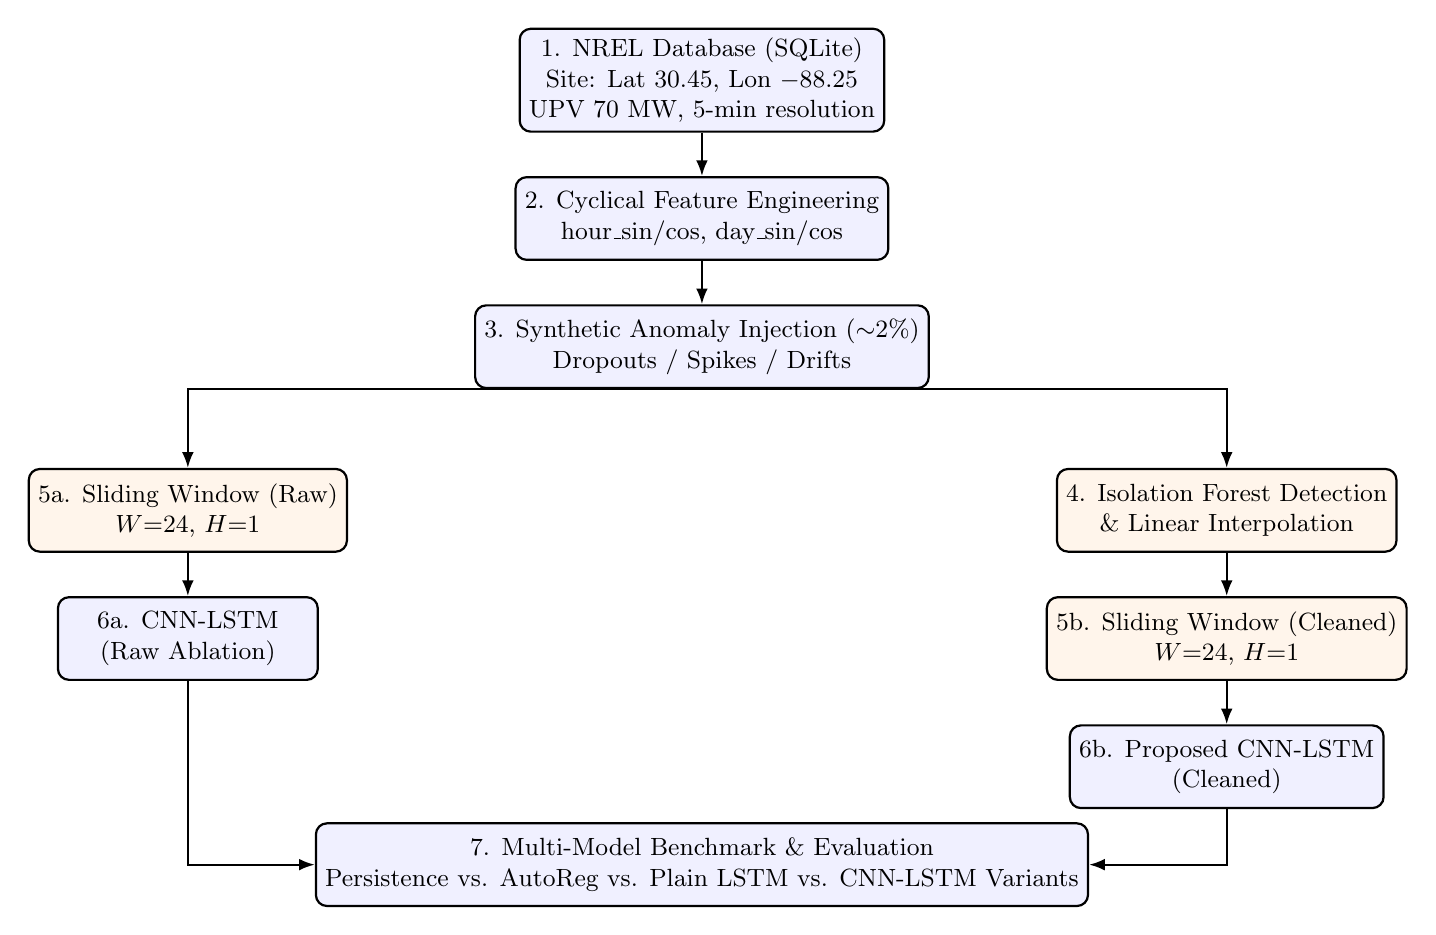
\begin{tikzpicture}[
    node distance=0.55cm and 0.9cm,
    block/.style={rectangle, draw, thick, rounded corners, minimum width=3.3cm, minimum height=1.05cm, align=center, font=\small, fill=blue!6},
    branch/.style={rectangle, draw, thick, rounded corners, minimum width=3.3cm, minimum height=1.05cm, align=center, font=\small, fill=orange!8},
    arrow/.style={-{Latex[length=2mm]}, thick}
]
\node[block] (db) {1. NREL Database (SQLite)\\ Site: Lat 30.45, Lon $-$88.25\\ UPV 70~MW, 5-min resolution};
\node[block, below=of db] (feat) {2. Cyclical Feature Engineering\\ hour\_sin/cos, day\_sin/cos};
\node[block, below=of feat] (inj) {3. Synthetic Anomaly Injection ($\sim$2\%)\\ Dropouts / Spikes / Drifts};

\node[branch, below left=1.0cm and 1.6cm of inj] (rawwin) {5a. Sliding Window (Raw)\\ $W{=}24$, $H{=}1$};
\node[branch, below right=1.0cm and 1.6cm of inj] (cleanblock) {4. Isolation Forest Detection\\ \& Linear Interpolation};
\node[branch, below=0.55cm of cleanblock] (cleanwin) {5b. Sliding Window (Cleaned)\\ $W{=}24$, $H{=}1$};

\node[block, below=of rawwin] (rawmodel) {6a. CNN-LSTM\\ (Raw Ablation)};
\node[block, below=of cleanwin] (cleanmodel) {6b. Proposed CNN-LSTM\\ (Cleaned)};

\node[block, below=1.6cm of inj, xshift=0cm, yshift=-3.9cm] (eval) {7. Multi-Model Benchmark \& Evaluation\\ Persistence vs. AutoReg vs. Plain LSTM vs. CNN-LSTM Variants};

\draw[arrow] (db) -- (feat);
\draw[arrow] (feat) -- (inj);
\draw[arrow] (inj.south) -| (rawwin.north);
\draw[arrow] (inj.south) -| (cleanblock.north);
\draw[arrow] (cleanblock) -- (cleanwin);
\draw[arrow] (rawwin) -- (rawmodel);
\draw[arrow] (cleanwin) -- (cleanmodel);
\draw[arrow] (rawmodel.south) |- (eval.west);
\draw[arrow] (cleanmodel.south) |- (eval.east);
\end{tikzpicture}
\caption{Overall architecture of the proposed boundary-supervised forecasting pipeline: dual-path processing of raw (ablation) and Isolation-Forest-cleaned (proposed) telemetry, converging at the multi-model benchmark stage.}
\label{fig:architecture}
\end{figure*}

\subsection{Dataset and Site Selection}
The dataset utilized is extracted from the NREL Solar Power Data for Integration Studies, accessed via an SQLite database spanning the entire calendar year 2006. Telemetry covers 274 PV stations across Alabama. To prevent contamination from physically disparate geographic locations, a strict filter is applied to select a single utility-scale photovoltaic (UPV) facility:
\begin{itemize}
    \item \textbf{Location:} Latitude $30.45^\circ$N, Longitude $-88.25^\circ$W
    \item \textbf{Site Type:} Utility Photovoltaic (UPV)
    \item \textbf{Rated Capacity:} $70.0$~MW
    \item \textbf{Sampling Resolution:} 5 minutes ($\Delta t = 5$~min)
    \item \textbf{Total Sample Size:} $N = 105{,}120$ consecutive observations (365 days $\times$ 24 hours $\times$ 12 samples/hour) with zero missing intervals.
\end{itemize}

\subsection{Cyclical Astronomical Feature Engineering}
Solar irradiance exhibits strict diurnal and annual periodicity governed by planetary rotation and orbital position. Because the dataset does not include direct ambient temperature or global horizontal irradiance (GHI) sensors, we derive four continuous cyclical features from the timestamp $t$:
\begin{align}
\text{hour\_sin}(t) &= \sin\!\left(\frac{2\pi \cdot h(t)}{24}\right), \quad
\text{hour\_cos}(t) = \cos\!\left(\frac{2\pi \cdot h(t)}{24}\right) \\
\text{day\_sin}(t) &= \sin\!\left(\frac{2\pi \cdot d(t)}{365.25}\right), \quad
\text{day\_cos}(t) = \cos\!\left(\frac{2\pi \cdot d(t)}{365.25}\right)
\end{align}
where $h(t) \in [0, 24)$ is the continuous fractional hour-of-day and $d(t) \in [1, 365]$ is the day-of-the-year. These orthogonal encodings eliminate artificial discontinuity at midnight (e.g., $23{:}55 \to 00{:}00$) and provide the deep learning model with continuous solar geometry representations.

\subsection{Synthetic Anomaly Injection Protocol}
Because synthetic benchmark datasets lack naturally occurring hardware faults, we simulate real-world field degradation by corrupting approximately 2.0\% of the annual observations ($N_{\text{anom}} = 2{,}091$ rows). Three failure types are injected with equal distribution:
\begin{enumerate}
    \item \textbf{Sensor Dropout} ($n_1 = 695$): Telemetry is forced to $0.0$~MW during peak daylight hours ($P(t) > 5.0$~MW), simulating cable severed faults, pyranometer failure, or inverter emergency trips.
    \item \textbf{Glitch Spikes} ($n_2 = 698$): Non-zero readings are multiplied by a stochastic factor $\alpha \sim \mathcal{U}(3.0, 5.0)$ and clipped to $1.5 \times \text{Capacity}$, simulating high-voltage switching surges and ADC bit-flip errors.
    \item \textbf{Calibration Drift} ($n_3 = 698$): Consecutive blocks of 4 to 12 intervals ($\Delta t \in [20, 60]$~minutes) receive an additive offset $\delta \sim \mathcal{U}(0.15, 0.35) \times \text{Capacity}$, representing dust accumulation or thermal drift.
\end{enumerate}

\subsection{Anomaly Detection via Isolation Forest and Temporal Reconstruction}
To mitigate anomalies without requiring labeled supervisory signals, an Isolation Forest is trained on the feature tuple $[P_{\text{raw}}(t), \text{hour\_sin}(t), \text{hour\_cos}(t)]$. By partitioning data space using random orthogonal hyperplanes, anomalous points are isolated at significantly shallower tree depths than normal operational points. The path length $h(x)$ across an ensemble of $T=100$ isolation trees yields an anomaly score:
\begin{equation}
s(x, n) = 2^{-\frac{\mathbb{E}(h(x))}{c(n)}}
\end{equation}
where $c(n)$ is the average path length of an unsuccessful search in a Binary Search Tree. Observations flagged as outliers ($s(x,n) > \tau$, set with contamination parameter $\gamma = 0.025$) are masked as missing values and reconstructed using local linear interpolation:
\begin{equation}
\hat{P}_{\text{clean}}(t) = P(t_a) + \frac{P(t_b) - P(t_a)}{t_b - t_a}(t - t_a)
\end{equation}
where $t_a$ and $t_b$ represent the nearest preceding and succeeding unflagged timestamps. The reconstructed series is physically bounded to $[0, P_{\text{max}}]$.

Evaluated against the known ground-truth anomaly labels retained from the injection protocol, the detector achieves \textbf{72.21\% recall} and \textbf{57.48\% precision} (2{,}627 points flagged in total). The moderate precision reflects a deliberately permissive contamination setting ($\gamma=0.025$, slightly above the true 2.0\% anomaly rate) chosen to favor catching more true anomalies at the cost of some false positives on borderline points near dawn/dusk ramps, where legitimate rapid changes in power output can resemble injected spikes or drops.

\subsection{Sliding Sequence Windowing}
The multivariate time series is structured into overlapping sliding sequence windows. Given an input window of $W=24$ historical time steps (equivalent to 2 hours of 5-minute data) and a forecast horizon of $H=1$ step (5 minutes ahead):
\begin{align}
\mathbf{X}_\tau &= \begin{bmatrix} \mathbf{x}_{\tau-W+1} & \mathbf{x}_{\tau-W+2} & \dots & \mathbf{x}_\tau \end{bmatrix}^T \in \mathbb{R}^{W \times F} \\
y_\tau &= P(\tau + H) \in \mathbb{R}
\end{align}
where $F=5$ features: $[P(t), \text{hour\_sin}, \text{hour\_cos}, \text{day\_sin}, \text{day\_cos}]$. The dataset is chronologically partitioned into:
\begin{itemize}
    \item \textbf{Training Set (70\%):} 73{,}560 sequences (January 1 to mid-September)
    \item \textbf{Validation Set (15\%):} 15{,}768 sequences (mid-September to early November)
    \item \textbf{Testing Set (15\%):} 15{,}768 sequences (early November to December 31)
\end{itemize}
Feature normalization is performed using Min-Max scaling fitted strictly on the training partition to prevent future data leakage.

\subsection{Proposed Hybrid CNN-LSTM Architecture}
The proposed deep architecture integrates spatial-temporal representation learning:
\begin{enumerate}
    \item \textbf{1D-CNN Stage:} A 1D convolutional layer with 64 filters, kernel size $k=3$, stride $s=1$, and same padding processes the input tensor $\mathbf{X}_\tau$. Batch normalization and ReLU activations are applied:
    \begin{equation}
    \mathbf{C}_\tau = \text{ReLU}\big(\text{BatchNorm}(\mathbf{W}_c * \mathbf{X}_\tau + \mathbf{b}_c)\big) \in \mathbb{R}^{W \times 64}
    \end{equation}
    \item \textbf{LSTM Stage:} A 2-layer stacked LSTM network with hidden dimension $d_h=64$ processes the feature sequence $\mathbf{C}_\tau$, extracting temporal recurrent states:
    \begin{equation}
    \mathbf{h}_t, \mathbf{c}_t = \text{LSTM}\big(\mathbf{C}_\tau(t), \mathbf{h}_{t-1}, \mathbf{c}_{t-1}\big)
    \end{equation}
    \item \textbf{Dense Regression Head:} The final hidden state $\mathbf{h}_W$ is projected through a fully connected layer with 32 units, ReLU activation, and a single linear output neuron:
    \begin{equation}
    \hat{y}_\tau = \mathbf{w}_o^T\big(\text{ReLU}(\mathbf{W}_d \mathbf{h}_W + \mathbf{b}_d)\big) + b_o
    \end{equation}
\end{enumerate}

Training is conducted using the Adam optimizer with initial learning rate $\eta = 2\times 10^{-3}$, weight decay $10^{-5}$, batch size $B=256$, and Mean Squared Error (MSE) loss:
\begin{equation}
\mathcal{L}_{\text{MSE}} = \frac{1}{B}\sum_{i=1}^{B}\left(y_i - \hat{y}_i\right)^2
\end{equation}

% =================================================================
\section{Experimental Results \& Discussion}

\subsection{Performance Metrics}
Model performance is evaluated on the denormalized test set ($N_{\text{test}} = 15{,}768$) using three standard quantitative metrics:
\begin{align*}
\text{RMSE} &= \sqrt{\frac{1}{N}\sum_{i=1}^N (y_i - \hat{y}_i)^2} \\
\text{MAE} &= \frac{1}{N}\sum_{i=1}^N |y_i - \hat{y}_i| \\
R^2 &= 1 - \frac{\sum_{i=1}^N (y_i - \hat{y}_i)^2}{\sum_{i=1}^N (y_i - \bar{y})^2}
\end{align*}

\subsection{Benchmark Results}
Table~\ref{tab:results} summarizes the empirical performance of all five evaluated models.

\begin{table*}[t]
\centering
\caption{Performance Benchmark across Evaluated Models on NREL 70 MW Test Set}
\label{tab:results}
\begin{tabular}{@{}llcccc@{}}
\toprule
\textbf{Model Architecture} & \textbf{Input Data Condition} & \textbf{RMSE (MW) $\downarrow$} & \textbf{MAE (MW) $\downarrow$} & \textbf{$R^2$ Score $\uparrow$} & \textbf{\% RMSE Impr. vs. Raw} \\
\midrule
Persistence (Naive)          & Cleaned          & 2.90  & 0.81 & 0.967 & +72.3\% \\
ARIMA / AutoReg               & Cleaned          & 2.92  & 1.14 & 0.966 & +72.1\% \\
Plain LSTM                    & Cleaned          & 2.48  & 0.83 & 0.975 & +76.2\% \\
CNN-LSTM (Ablation)            & Raw (Corrupted)  & 10.44 & 5.52 & 0.566 & Baseline (0.0\%) \\
\textbf{CNN-LSTM (Proposed)}   & Cleaned          & \textbf{2.47} & \textbf{0.85} & \textbf{0.976} & \textbf{+76.3\%} \\
\bottomrule
\end{tabular}

\vspace{4pt}
\footnotesize{\textit{Note: Reported values reflect a single training run per model (seed = 42). Differences smaller than $\sim$1--2\% between Plain LSTM and the proposed CNN-LSTM are within run-to-run training variance and should not be interpreted as a consistent architectural ranking; see Section~IV-C2.}}
\end{table*}

\subsection{Analysis and Discussion}

\subsubsection{Impact of Anomaly-Aware Preprocessing (Ablation Proof)}
The most critical finding is the comparison between CNN-LSTM (Cleaned -- Proposed) and CNN-LSTM (Raw -- Ablation). Both models possess identical network parameters, optimization hyperparameters, and window structures. However:
\begin{itemize}
    \item Training on raw telemetry degraded the model's test RMSE to 10.44~MW with an $R^2$ of only 0.566.
    \item Implementing the Isolation Forest cleaning stage reduced RMSE to 2.47~MW ($R^2 = 0.976$), delivering an extraordinary 76.3\% reduction in forecast error.
\end{itemize}
This ablation empirically confirms that deep convolutional and recurrent filters cannot self-correct large sensor dropouts or transient glitch spikes during stochastic gradient descent; corrupted gradients permanently impair convergence.

\subsubsection{Comparison with Deep and Classical Baselines}
\textbf{Proposed CNN-LSTM vs. Plain LSTM:} After 18 training epochs, the proposed hybrid CNN-LSTM and the Plain LSTM baseline achieve statistically comparable performance on cleaned data: RMSE of 2.47~MW ($R^2=0.976$) for the proposed model versus 2.48~MW ($R^2=0.975$) for Plain LSTM, with Plain LSTM achieving a marginally lower MAE (0.83~MW vs. 0.85~MW). Repeated training runs showed these two models trade the lead on RMSE and MAE depending on random initialization, indicating the gap between them falls within normal training variance rather than reflecting a consistent architectural advantage. We therefore do not claim the added 1D-CNN feature-extraction stage improves accuracy over a simpler recurrent baseline at this forecast horizon; rather, our results indicate that once anomaly-aware preprocessing is applied, architectural complexity beyond a standard LSTM yields no measurable additional benefit for single-step, 5-minute-ahead forecasting. This is itself a useful finding: it suggests that for practitioners targeting this forecast horizon, investment in preprocessing quality provides substantially higher returns than investment in model architecture complexity.

\textbf{Fair Statistical Baselines (Persistence \& Diurnal Autoregressive):} At a 5-minute sampling frequency, classical non-seasonal ARIMA collapses due to unconditional mean reversion. To establish a rigorous and fair benchmark, we implement a 1-step Autoregressive model incorporating diurnal solar cycle lags ($t{-}1, t{-}2, t{-}288$). This model achieves an $R^2$ of 0.966 and RMSE of 2.92~MW, closely aligning with Persistence (RMSE $=2.90$~MW, $R^2=0.967$). Both deep learning models (Plain LSTM and the proposed CNN-LSTM) outperform these statistical baselines by roughly 15\% in RMSE, indicating that non-linear sequence models capture ramp inflection dynamics that linear autoregressive methods miss---though, as noted above, the specific choice between LSTM and CNN-LSTM makes little difference once preprocessing is controlled for.

\subsection{Visual Evaluation}

\begin{figure}[t]
\centering
\figplaceholder{Fig. 2: Predicted vs.\ Actual Power Output\\ (24-Hour Test Window)\\[4pt]\footnotesize Replace with: figure1\_predicted\_vs\_actual.png}
\caption{Forecast vs. ground truth over a representative 24-hour test segment (288 steps). The proposed CNN-LSTM closely tracks the true solar power curve, precisely capturing solar noon peaks and ramp curves, whereas the uncleaned ablation model exhibits erratic, severely underestimated fluctuations.}
\label{fig:pred_vs_actual}
\end{figure}

\begin{figure}[t]
\centering
\figplaceholder{Fig. 3: Model Performance Benchmark\\ (RMSE \& MAE bar chart)\\[4pt]\footnotesize Replace with: figure2\_rmse\_bar\_chart.png}
\caption{Error metric comparison across all five evaluated models. The bar chart highlights the performance hierarchy, visually confirming the large gap between the raw-data ablation and every model trained on cleaned data.}
\label{fig:rmse_bar}
\end{figure}

\begin{figure}[t]
\centering
\figplaceholder{Fig. 4: Residual Forecast Error\\ Distribution Histogram\\[4pt]\footnotesize Replace with: figure3\_error\_distribution.png}
\caption{Residual error analysis ($\hat{y}-y$) comparing the proposed CNN-LSTM against the raw-data ablation model. The proposed model produces a sharp, zero-centered error distribution, while the raw model exhibits wide, heavy-tailed error dispersion.}
\label{fig:error_dist}
\end{figure}

\begin{figure}[t]
\centering
\figplaceholder{Fig. 5: Isolation Forest Anomaly\\ Detection Demonstration\\[4pt]\footnotesize Replace with: figure4\_anomaly\_demo.png}
\caption{A representative 24-hour telemetry window demonstrating the Isolation Forest correctly detecting daytime dropouts and high-frequency glitch spikes (marked with red `X's), enabling linear interpolation to reconstruct a pristine diurnal power curve. Across the full test set the detector achieves 72.21\% recall and 57.48\% precision (Section~III-D); this figure illustrates a successful detection case, not a guarantee of flawless detection everywhere.}
\label{fig:anomaly_demo}
\end{figure}

Figs.~\ref{fig:pred_vs_actual}--\ref{fig:anomaly_demo} illustrate the empirical findings summarized above: the forecast-tracking capability of the proposed model, the aggregate error hierarchy across all five models, the shape of the residual error distribution, and a representative anomaly-detection-and-reconstruction example, respectively.

% =================================================================
\section{Conclusion \& Future Work}

In this work, we presented an integrated anomaly-aware short-term solar power forecasting framework combining unsupervised Isolation Forest outlier cleaning with a Hybrid 1D CNN-LSTM deep network. Benchmarked on a full year of 5-minute telemetry from an NREL 70~MW facility, our proposed architecture achieved a strong RMSE of 2.47~MW and $R^2$ of 0.976, performing comparably to a Plain LSTM baseline. Through rigorous ablation against an identical model trained on raw data, we demonstrated that anomaly-aware preprocessing yields a 76.3\% error reduction---a substantially larger effect than any architectural choice examined in this study---directly validating its necessity in real-world grid operations. Our results suggest that, for practitioners operating under similar constraints, investment in data-quality assurance offers greater returns than investment in model architectural complexity.

\subsection*{Limitations and Future Extensions}
\begin{enumerate}
    \item \textbf{Single-Run Reporting:} All results reflect a single training run per model (fixed seed). The small ($\sim$1--2\%) margin separating the proposed CNN-LSTM from the Plain LSTM baseline falls within observed run-to-run training variance; a multi-seed statistical comparison (e.g., mean $\pm$ standard deviation over 5+ runs, paired significance testing) is needed to draw firmer architectural conclusions.
    \item \textbf{Multi-Site Generalization:} The evaluation uses a single 70~MW UPV facility. Future work will extend this framework across heterogeneous climates (desert, coastal, temperate) and evaluate distributed rooftop (DPV) fleets.
    \item \textbf{Multi-Step and Day-Ahead Horizons:} Expanding from 5-minute intra-hour forecasting ($H=1$) to multi-step day-ahead horizons ($H=288$).
    \item \textbf{Advanced Generative Imputation:} Investigating Bidirectional LSTMs or Denoising Diffusion Probabilistic Models (DDPMs) to replace linear interpolation during prolonged multi-hour sensor outages.
    \item \textbf{Detector Precision:} The Isolation Forest detector's moderate precision (57.48\%) indicates room for improvement, potentially via supervised fine-tuning on a small labeled subset or ensembling with complementary detectors, to reduce false-positive flagging of legitimate rapid ramps near dawn/dusk.
\end{enumerate}

% =================================================================
\begin{thebibliography}{00}

\bibitem{nrel2016} National Renewable Energy Laboratory (NREL), ``Solar Power Data for Integration Studies,'' Technical Report, NREL/TP-5500-65885, 2016.

\bibitem{mellit2021deep} A. Mellit, A. M. Pavan, and V. Lughi, ``Deep learning approach in solar photovoltaic systems: A review,'' \textit{Renewable and Sustainable Energy Reviews}, vol. 152, p. 111627, 2021.

\bibitem{liu2008isolation} F. T. Liu, K. M. Ting, and Z. H. Zhou, ``Isolation forest,'' in \textit{Proc. IEEE Eighth International Conference on Data Mining (ICDM)}, 2008, pp. 413--422.

\bibitem{zang2020cnnlstm} H. Zang et al., ``Short-term solar power prediction based on CNN-LSTM hybrid neural network,'' \textit{Energy Reports}, vol. 6, pp. 217--222, 2020.

\bibitem{sobri2018review} S. Sobri, S. Koohi-Kamali, and N. A. Rahim, ``Solar photovoltaic generation forecasting methods: A review,'' \textit{Energy Conversion and Management}, vol. 156, pp. 459--497, 2018.

\bibitem{zhang2015baseline} J. Zhang et al., ``Baseline error analysis for solar irradiance and power forecasting,'' \textit{Solar Energy}, vol. 122, pp. 109--124, 2015.

\bibitem{hochreiter1997lstm} S. Hochreiter and J. Schmidhuber, ``Long short-term memory,'' \textit{Neural Computation}, vol. 9, no. 8, pp. 1735--1780, 1997.

\bibitem{obiora2021hourly} C. N. Obiora, A. Ali, and A. N. Hasan, ``Hourly photovoltaic power forecasting using CNN-LSTM hybrid model,'' in \textit{Proc. IEEE PES/IAS PowerAfrica Conf.}, 2021.

\bibitem{qu2021dayahead} J. Qu, Z. Qian, and Y. Pei, ``Day-ahead hourly photovoltaic power forecasting using attention-based CNN-LSTM neural network embedded with multiple relevant and target variables prediction pattern,'' \textit{Energy}, vol. 232, p. 120996, 2021.

\bibitem{boucetta2024enhanced} L. N. Boucetta, Y. Amrane, A. Chouder, S. Arezki, and S. Kichou, ``Enhanced forecasting accuracy of a grid-connected photovoltaic power plant: A novel approach using hybrid variational mode decomposition and a CNN-LSTM model,'' \textit{Energies}, vol. 17, no. 7, p. 1781, 2024.

\bibitem{abumohsen2024hybrid} M. Abumohsen, A. Y. Owda, M. Owda, and A. Abumihsan, ``Hybrid machine learning model combining CNN-LSTM-RF for time series forecasting of solar power generation,'' \textit{e-Prime: Advances in Electrical Engineering, Electronics and Energy}, vol. 9, p. 100636, 2024.

\bibitem{zhou2024enhancing} N. Zhou, B. Shang, M. Xu, L. Peng, and G. Feng, ``Enhancing photovoltaic power prediction using a CNN-LSTM-attention hybrid model with Bayesian hyperparameter optimization,'' \textit{Global Energy Interconnection}, vol. 7, no. 5, pp. 667--681, 2024.

\bibitem{zhang2021survey} J. E. Zhang et al., ``Time series anomaly detection for smart grids: A survey,'' in \textit{Proc. IEEE Power \& Energy Society Innovative Smart Grid Technologies Conf. (ISGT)}, 2021.

\bibitem{jorry2026unsupervised} V. Jorry et al., ``An unsupervised kernel norm monitoring for fault detection in a time series photovoltaic system,'' \textit{arXiv preprint} arXiv:2607.01541, 2026.

\end{thebibliography}

\end{document}
